\documentclass[number]{ximera}

%My github password is ximera1
%My GeoGebra password is Ximera1

% set font encoding for PDFLaTeX, XeLaTeX, or LuaTeX
\usepackage{ifxetex,ifluatex}
\newif\ifxetexorluatex
\ifxetex
  \xetexorluatextrue
\else
  \ifluatex
    \xetexorluatextrue
  \else
    \xetexorluatexfalse
  \fi
\fi

\ifxetexorluatex
  \usepackage{fontspec}
\else
  \usepackage[T1]{fontenc}
  \usepackage[utf8]{inputenc}
  \usepackage{lmodern}
\fi

\usepackage{hyperref}

\usepackage{tikz}

\title{Area of a Triangle}
\author{Univ. of Minnesota MathCEP}


% Enable SageTeX to run SageMath code right inside this LaTeX file.
% http://mirrors.ctan.org/macros/latex/contrib/sagetex/sagetexpackage.pdf
% \usepackage{sagetex}

\begin{document}

\begin{abstract}
  In this activity, you will discover additional formulas for calculating the area of a triangle in the SAS case and when two angles and a side length are given. The SSS case can be done in a similar manner, though the most common form, called {\it{Heron's Formula}} is not easily derived.
\end{abstract}

\maketitle

Assume we know the formula for the area of a triangle

$$Area \; = \; \frac{1}{2}(base)(height)$$

\begin{enumerate}

\item (SAS) Do as many of the following problems as are necessary for you to develop a process that you can describe in question 2. In each case, find $h$ and the area of the triangle. Note that $b$ is the entire length from $A$ to $C$, not just the portion that would be the adjacent side to angle $A$ in the right triangle.

\begin{enumerate}

\item Given $b = 7$, $c=5$ and $A = 35^\circ$, find $h$ and the area of the triangle.

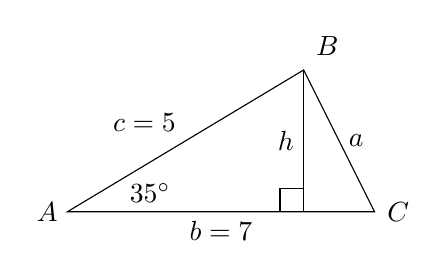
\begin{tikzpicture}[scale=3]


\draw node[left]{$A$} (0,0) -- node[below] {$b=7$} (1.3,0) -- node[right] {$a$}  (1,0.6) -- node[above left] {$c=5$} (0,0) -- cycle;

\draw (1,0.6) -- node[left]{$h$} (1,0);
\draw (0.9,0.1) -- (0.9,0);
\draw (0.9,0.1) -- (1,0.1);
\node at (1.1,0.7) {$B$};
\node at (1.4,0) {$C$};
\node at (0.35,0.08) {$35^\circ$};

\end{tikzpicture}
 
\item Given $b = 12$, $c=8$ and $A = 52^\circ$, find $h$ and the area of the triangle.
\item Given $b = 4$, $c=11$ and $A = 83^\circ$, find $h$ and the area of the triangle.
\item Given $b = 10$, $c=9$ and $A = 115^\circ$, find $h$ and the area of the triangle.
 
\end{enumerate}
 
\item Describe, in words, the steps needed to find the area of a triangle, given $A$, $b$, and $c$. (You may also use mathematical expressions in your description.)

\item Using $c$ and $A$, write a formula for $h$. Then write a formula for the area of the triangle. 

 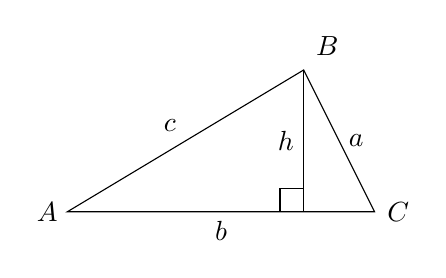
\begin{tikzpicture}[scale=3]


\draw node[left]{$A$} (0,0) -- node[below] {$b$} (1.3,0) -- node[right] {$a$}  (1,0.6) -- node[above left] {$c$} (0,0) -- cycle;

\draw (1,0.6) -- node[left]{$h$} (1,0);
\draw (0.9,0.1) -- (0.9,0);
\draw (0.9,0.1) -- (1,0.1);
\node at (1.1,0.7) {$B$};
\node at (1.4,0) {$C$};
 \end{tikzpicture}
 
\item Repeat using $a$ and $C$. That is, using $a$ and $C$, write a formula for $h$. Then write a formula for the area of the triangle.

\newpage

\item (AAS = AAAS = ASA) Do as many of the following problems as are necessary for you to develop a process that you can describe in question 6. In each case, find $c$, then find $h$, then find the area of the triangle. Note that $b$ is the entire length from $A$ to $C$, not just the portion that would be the adjacent side to angle $A$ in the right triangle.

\begin{enumerate}

\item Given $b = 7$, $A = 35^\circ$, $B = 65^\circ$ and $C = 80^\circ$

 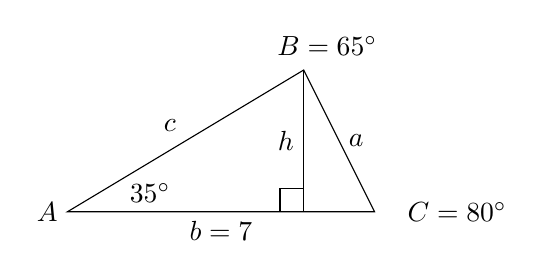
\begin{tikzpicture}[scale=3]

\draw node[left]{$A$} (0,0) -- node[below] {$b=7$} (1.3,0) -- node[right] {$a$}  (1,0.6) -- node[above left] {$c$} (0,0) -- cycle;

\draw (1,0.6) -- node[left]{$h$} (1,0);
\draw (0.9,0.1) -- (0.9,0);
\draw (0.9,0.1) -- (1,0.1);
\node at (1.1,0.7) {$B=65^\circ$};
\node at (1.65,0) {$C=80^\circ$};
\node at (0.35,0.08) {$35^\circ$};

 \end{tikzpicture}
 
 \begin{itemize}
\item Find $c$

\item Find $h$

\item Find the area of the triangle
 
 \end{itemize}
 
 \item Given $b = 12$, $A = 52^\circ$, $B = 67^\circ$ and $C = 61^\circ$

\item Given $b = 5$, $A = 85^\circ$, $B = 23^\circ$ and $C = 72^\circ$

\item Given $b = 11$, $A = 115^\circ$, $B = 43^\circ$ and $C = 22^\circ$
 
 \end{enumerate}
 
 \item Describe, in words, the steps needed to find the area of a triangle, given $b$, $A$, $B$, and $C$. (You may also use mathematical expressions in your description.)
 
\item Derive a formula for the area of a triangle, given $b$, $A$, $B$ and $C$, by doing the following

 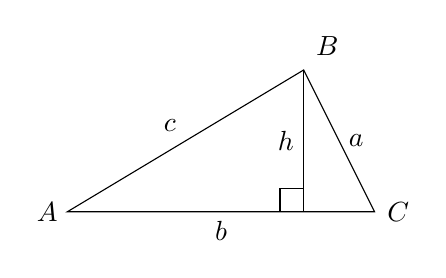
\begin{tikzpicture}[scale=3]


\draw node[left]{$A$} (0,0) -- node[below] {$b$} (1.3,0) -- node[right] {$a$}  (1,0.6) -- node[above left] {$c$} (0,0) -- cycle;

\draw (1,0.6) -- node[left]{$h$} (1,0);
\draw (0.9,0.1) -- (0.9,0);
\draw (0.9,0.1) -- (1,0.1);
\node at (1.1,0.7) {$B$};
\node at (1.4,0) {$C$};
 \end{tikzpicture}


 
  \begin{itemize}
\item Find $c$, as a function of $b$, $C$ and $B$ 

\item Find $h$, as a function of $c$ and $A$

\item Find $h$, as a function of $b$, $A$, $B$ and $C$

\item Find the area of the triangle, as a function of $b$, $A$, $B$ and $C$
 
 \end{itemize}
 

\end{enumerate}
\end{document}


\end{document}
